\section*{Executive Summary}
\noindent
This project applies the CRISP-DM process to housing listing data covering the USA (no territories are included). The stated goal is twofold: to predict property price and %to identify which property features appear to affect market value. %\hl{The intended audience includes buyers, sellers, listing and buyer agents, brokers, mortgage lenders, homeowners, and renters.} 
identify important features that affect market value. %The intended audience primarily focuses on buyers and sellers.
The target audience is mainly buyers and sellers.

\\
\noindent
%\hl{According to the project pages, the dataset was obtained from Kaggle and was described there as housing listings scraped from Craigslist around January 2020. The original file is a CSV with 384,977 rows, 22 columns, and a size of 558.44 MB. The target variable for modeling is price.} 
The dataset was obtained from \href{https://www.kaggle.com/datasets/austinreese/usa-housing-listings}{Kaggle} and was scraped from Craigslist around January 2020.\\
\noindent
The data understanding and preparation work focused on %describing the variables, identifying missing values, removing unsuitable records, handling price outliers with an IQR-based approach at the region level, and 
describing and cleaning the dataset (Regional IQR Price Outliers)
%and constructing a new location-based feature called \texttt{location\_cluster} using K-Means clustering on latitude and longitude. 
and attempting to cluster \textit{lat.}\&\textit{long.} points around cities/metropolitan areas using K-Means. %\\
%\noindent
For modeling, the project used Random Forest, HistGradientBoosting, and XGBoost. Tree-based models were selected based on EDA.

%, with the tree-based model selection based on the exploratory analysis.

%with the heatmap observation used to justify tree-based methods over a simple linear approach. 
%\hl{The project notes also state that adding location clustering improved results, and that region-level outlier treatment performed better than applying a single IQR rule to the entire country.} 
\\
\noindent
The overall conclusion recorded in the project pages is that the models performed well on average, but the final recommendation is revision rather than deployment. Suggested next steps include tuning the number of location clusters, collecting more data, exploring GPU-accelerated boosting implementations, and using NLP or transformer methods on the description field. %\href{https://www.kaggle.com/datasets/austinreese/usa-housing-listings}{1}


%\noindent
%
\includegraphics[width=\textwidth,height=\textheight-35\baselineskip,keepaspectratio]{Assignment/week14/charts/CRISP-DM.png}\\

\begin{figure}[ht!]
  \centering
  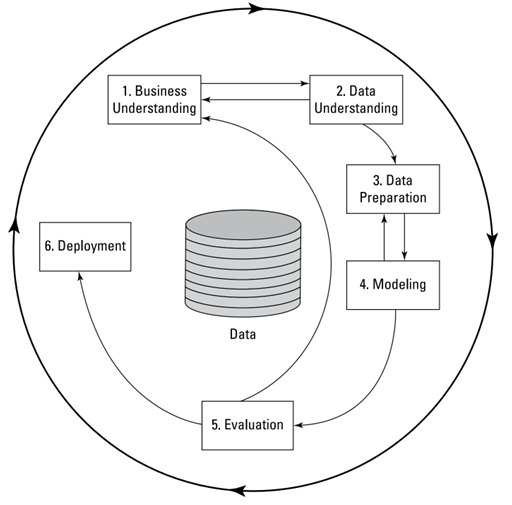
\includegraphics[height=250pt]{Assignment/Phase1-5_new/charts/CRISP-DM.png}
  \caption{CRISP-DM pipeline diagram}
  \label{fig:CRISP-DM pipeline diagram}
\end{figure}


%try